\documentclass{article}
\usepackage[utf8]{inputenc}
\usepackage{hyperref}
\usepackage[letterpaper, portrait, margin=1in]{geometry}
\usepackage{enumitem}
\usepackage{amsmath}
\usepackage{amsthm}
\usepackage{booktabs}
\usepackage{graphicx}
\usepackage{float}
\usepackage{hyperref}
\usepackage[flushleft]{threeparttable}
\usepackage{textcomp}
\usepackage{amssymb}
\usepackage{dsfont}
\hypersetup{
colorlinks=true,
    linkcolor=black,
    filecolor=black,      
    urlcolor=blue,
    citecolor=black,
}
\usepackage{natbib}
\usepackage{yhmath}

\usepackage{titlesec}
\bibliographystyle{chicago}
\newcommand{\bib}{references.bib}
\newcommand\iid{\stackrel{\mathclap{iid}}{\sim}}
\newcommand\asym{\stackrel{\mathclap{a}}{\sim}}
\newcommand\convprob{\xrightarrow{p}}
\newcommand\convdist{\xrightarrow{d}}
\newcommand{\N}{\mathbb{N}}
\newcommand{\Z}{\mathbb{Z}}
\newcommand{\E}{\text{E}}
\newcommand{\V}{\text{Var}}
\newcommand{\Av}{\text{Avar}}
\newcommand{\se}{\text{se}}
\newcommand{\corr}{\text{Corr}}
\newcommand{\cov}{\text{Cov}}
\newcommand{\norm}{\text{Normal}}
\newcommand{\indep}{\perp \!\!\! \perp}

\begin{document}
% The tex content below is similar to the given main.tex
 
\title{Homework 8}
\author{Environmental Economics II\\
Maghfira Ramadhani}
\date{\today}
\maketitle

\section*{Problem 1 Stata}
\begin{enumerate}
\item Variable \verb!l_mw! and \verb!treatment! are generated.
\begin{enumerate}
    \item Using the specification in equation 1, the treatment effect estimate is -0.06560 with a standard error of 0.00136.
    \item The treatment effect estimate is -0.07039 with a standard error of 0.001. Following the Stata package documentation, it is recommended to use the bias-corrected estimator for two or more continuous control variables. Using the bias-corrected estimator, the treatment effect estimate is -0.08117 with a standard error of 0.00106. 
    \item I would suspect the COVID effect will make people to work from home and thus increase the electricity consumption. Methods used in 1(a) and 1(b) measure the treatment effect by comparing electricity consumption between the treated and untreated household within similar zone at the same month, day, and hour. Both do not capture the annual trend in electricity consumption. With 1(a) month 1 and 2 are never treated as COVID happen only from month 3 to 12 in the sample.
\end{enumerate}
\item The following estimates are obtained from estimating equation 2.
\begin{enumerate}
    \item The treatment effect estimate is 0.02356 with a standard error of 0.00271.
    \item Now that we capture the annual trend using equation 2, the treatment effect makes more sense.
\end{enumerate}
\begin{figure}[H]
    \centering
    %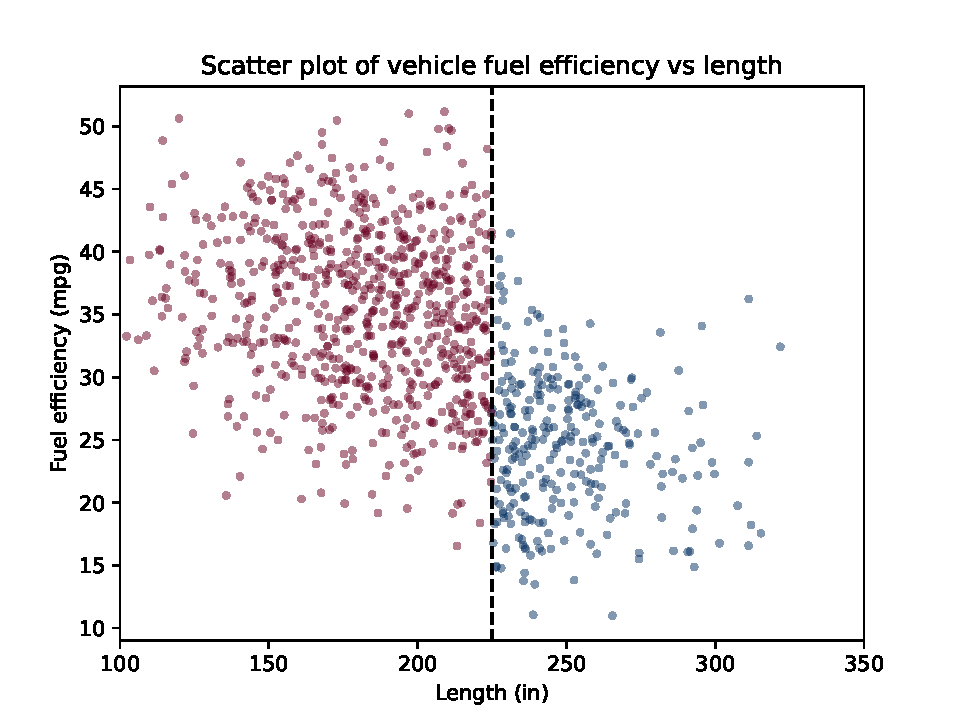
\includegraphics[width=0.4\textwidth]{./figure/scatterplot.pdf}
    \caption{Scatter plot of fuel efficiency vs length of vehicle}
    \label{f1:scatter_plot} 
\end{figure}
\item Table \ref{t:RD} shows the RD estimates for using different polynomial.
\begin{table}[H]\centering
    \caption{RD estimates}
    \label{t:RD}
    \begin{threeparttable}
    %\begin{tabular}{@{\extracolsep{5pt}}lccc}
\\[-1.8ex]\hline
\hline \\[-1.8ex]
& \multicolumn{3}{c}{\textit{Dependent variable: Fuel efficiency (mpg)}} \
\cr \cline{2-4}
\\[-1.8ex] & (1) & (2) & (3) \\
\hline \\[-1.8ex]
 LATE & -10.920$^{**}$ & -8.255$^{}$ & 0.376$^{}$ \\
& (4.495) & (46.302) & (0.342) \\
\hline \\[-1.8ex]
 Polynomial specification & 1$^{st}$ order & 2$^{nd}$ order & 5$^{th}$ order \\
 Observations & 1000 & 1000 & 1000 \\
 $R^2$ & 0.399 & 0.399 & 0.401 \\
 Adjusted $R^2$ & 0.397 & 0.396 & 0.395 \\
 Residual Std. Error & 6.158 & 6.160 & 6.165 \\
 F Statistic & 259.649$^{***}$ & 162.427$^{***}$ & 248.217$^{***}$ \\
\hline
\hline \\[-1.8ex]
\textit{Note:} & \multicolumn{3}{r}{$^{*}$p$<$0.1; $^{**}$p$<$0.05; $^{***}$p$<$0.01} \\
\end{tabular}
    \end{threeparttable}
    \end{table}
\end{enumerate}



\end{document}